% Paper 3 — definitional fragmentation in Saudi legislation.
% Venue-adaptive: uses a journal class when present, else a self-contained
% single-column fallback that compiles on a plain TeX Live.
\IfFileExists{sn-jnl.cls}{%
  \documentclass[sn-basic]{sn-jnl}%
  \newcommand{\usingsnstyle}{}%
}{%
  \documentclass[11pt]{article}%
  \usepackage[a4paper,top=2.5cm,bottom=2.5cm,left=3cm,right=3cm]{geometry}%
  \usepackage{times}%
  \usepackage[round]{natbib}%
  \usepackage{setspace}%
  \onehalfspacing%
  \usepackage[hidelinks]{hyperref}%
}

% Set \anontrue when the target journal reviews anonymously.
\newif\ifanon
\anonfalse

\usepackage[T1]{fontenc}
\usepackage[utf8]{inputenc}
\usepackage{microtype}
\usepackage{booktabs}
\usepackage{graphicx}
\usepackage{url}
\emergencystretch=3em

\title{What Counts as an Establishment? Measuring Definitional Fragmentation
Across Saudi Arabian Legislation}

\ifanon
  \author{}
  \date{}
\else
  \ifdefined\usingsnstyle
    \author*[1]{\fnm{Abdullah} \sur{Almohammedi}}\email{abdullah.m.almohammedi@gmail.com}
    \affil[1]{\orgname{Independent Researcher}}
  \else
    \author{Abdullah Almohammedi \\
      Independent Researcher \\
      \texttt{abdullah.m.almohammedi@gmail.com} \\
      ORCID: \href{https://orcid.org/0009-0001-0832-0995}{0009-0001-0832-0995}}
    \date{}
  \fi
\fi

\begin{document}

\maketitle

\begin{abstract}
Statutes define their terms, and different statutes define the same terms
differently. Whether that matters --- whether it represents genuine
inconsistency or merely the ordinary business of legislative drafting --- has
been argued from examples rather than measured. Using a machine-readable
corpus of 290 Saudi Arabian legislative instruments carrying 1{,}920 defined
terms and 3{,}318 definitions, we measure it. The measurement requires two
filters that the question's framing tends to hide. The first separates
\emph{indexical} definitions, in which an instrument defines ``the Law'' as
itself or ``the Ministry'' as its own supervising body: these are the most
frequently repeated definitions in the corpus, they are instrument-local by
construction, and they cannot disagree. They account for 171 of the 1{,}920
terms and dominate any raw ranking, the term ``the Law'' being defined 125
times. The second separates lexical from substantive divergence. Among the
322 substantive terms defined by more than one instrument, 61.5\% carry
definitions that diverge lexically --- a figure that would make a striking
headline and that we argue should not be read as legal inconsistency, since
the most widely shared term of all, ``person'', is defined by 27 instruments
in wording that varies while the meaning does not. Reading the twelve most
widely shared substantive terms across every instrument that defines them,
we find three harmonized, two with instrument-local referents, two indexical
cases the automatic filter missed, one instance of homonymy, and four
carrying materially conflicting scope --- so that within this sample lexical
divergence overstates substantive conflict roughly threefold. The clearest is
\emph{al-munsha'ah}, ``establishment'': under the Competition Law any person
carrying on an economic activity, under the Labour Law any undertaking
employing at least one worker for wages. A sole trader with no employees is
an establishment for one statute and not for the other. We conclude that
definitional fragmentation in Saudi legislation is real but far narrower
than automatic measurement suggests, that the distinction between lexical
and substantive divergence is the methodological crux for any jurisdiction,
and that the small set of genuinely conflicting terms is a tractable target
for legislative harmonisation and a necessary input for legal AI systems
that resolve statutory terms across instruments.
\end{abstract}

\ifdefined\usingsnstyle
\keywords{Statutory definitions, Legislative drafting, Saudi Arabia, Legal
informatics, Terminological consistency, Corpus methods}
\else
\vspace{1em}\noindent\textbf{Keywords:} Statutory definitions $\cdot$
Legislative drafting $\cdot$ Saudi Arabia $\cdot$ Legal informatics $\cdot$
Terminological consistency $\cdot$ Corpus methods
\vspace{1em}
\fi

\section{Introduction}

Legislative drafting manuals agree that a term should mean the same thing
throughout a legal system, and legislative practice does not comply. Statutes
define their own terms, definitions accumulate, and the same word ends up
carrying different content in different instruments. Practitioners encounter
this constantly; the literature discusses it through well-chosen examples.
What has been missing is measurement, and the reason is that measurement
requires a machine-readable corpus of statutory definitions, which few
jurisdictions have.

This paper measures definitional fragmentation across the legislation of
Saudi Arabia, using a corpus of 290 instruments in which every definitions
article has been parsed into term--definition pairs: 1{,}920 distinct terms
carrying 3{,}318 definitions \citep{almohammedi2026corpus}. The corpus makes
the question tractable for the first time in an Arab jurisdiction, and Saudi
Arabia is a useful case: its legislation was substantially rewritten in the
2020s, so definitions drafted decades apart now sit alongside definitions
drafted last year.

The central finding is negative in a way we think is more useful than a
striking positive would have been. Measured automatically, definitional
fragmentation looks severe: among substantive terms shared by more than one
instrument, 61.5\% carry lexically divergent definitions. Read by hand, most
of that divergence is not legal inconsistency at all. It is variation in
wording around a stable meaning, or homonymy, or a referent that each
instrument fixes for itself. The residue that does represent conflict is
small, specific, and --- because it is small and specific --- actionable.

Getting from the first number to the second requires two separations that
this paper treats as its methodological contribution.

The first is \emph{indexical} versus \emph{substantive} definitions. Saudi
instruments open by defining ``the Law'' as themselves, ``the Regulation'' as
their own implementing regulation, ``the Minister'' as whichever minister
supervises them. These are the most repeated definitions in the corpus ---
``the Law'' appears as a defined term in 125 instruments --- and they are
instrument-local by construction. Two instruments defining ``the Minister''
differently are not in conflict; they have different ministers. Any measure
that counts them produces a number about drafting convention rather than
about legal coherence.

The second is \emph{lexical} versus \emph{substantive} divergence.
Automatic similarity measures compare wording. Legal consistency is a
property of meaning. The term ``person'' is defined by 27 Saudi instruments,
in formulations ranging from ``the natural or legal person'' to ``any person
of natural or legal capacity, public or private''; lexical overlap between
some pairs is near zero and the legal content is identical. Reporting the
lexical figure as fragmentation would be, in a precise sense, measuring the
wrong thing.

Section~\ref{sec:method} sets out both separations and the hand-adjudication
procedure. Section~\ref{sec:results} reports what survives them.
Section~\ref{sec:discussion} argues that the surviving cases matter for
legislative harmonisation and for legal AI, and Section~\ref{sec:limits}
sets out what the method cannot see.

\section{Related work}

\paragraph{Statutory definitions.}
Definitions are a recognised topic in legislative drafting scholarship,
where the standard guidance is that a defined term should be used
consistently and that definitions should not vary between related
instruments without reason. The scholarship is largely doctrinal and
example-driven; corpus-scale measurement of whether a legal system actually
achieves definitional consistency is rare, and we are aware of none for an
Arab jurisdiction.

\paragraph{Legal informatics and legal corpora.}
Machine-readable legal corpora have grown substantially --- the Pile of Law
\citep{henderson2022pileoflaw}, MultiLegalPile
\citep{niklaus2024multilegalpile} --- but they are built for language-model
training rather than for structural analysis, and none covers Saudi
legislation. Structural standards such as Akoma Ntoso
\citep{palmirani2011akoma} model legislative documents without extracting
definitional content. The corpus used here \citep{almohammedi2026corpus}
ships a glossary layer that parses definitions articles into term--definition
pairs with provenance, which is what makes this study possible.

\paragraph{Quantitative studies of legal systems.}
Work measuring legal complexity and structure at corpus scale
\citep{katz2014complexity, coupette2021measuring} has concentrated on
citation and on document structure rather than on terminology. A companion
study analyses the citation network of the same corpus; the present paper
takes the complementary question of whether the instruments in that network
speak a common language.

\section{Data and method}
\label{sec:method}

\subsection{Corpus and glossary}

Saudi statutes conventionally open with a definitions article of the form
``the following words and phrases, wherever they appear in this Law, shall
have the meanings assigned to them''. A parser over those articles yields
1{,}920 distinct terms carrying 3{,}318 definitions, drawn from the 214
instruments whose definitions articles parse cleanly
\citep{almohammedi2026corpus}. Each definition record carries the term as
written, the definition text, the instrument, and the article it came from.

\subsection{Filter one: indexical definitions}

A definition is \emph{indexical} when it names a particular instrument or
organ of state rather than describing a class: ``the Law'' defined as ``the
Agriculture Law'', ``the Ministry'' as ``the Ministry of Environment, Water
and Agriculture''. Such definitions are local to the enacting instrument by
design and cannot be inconsistent with one another.

We detect them by a rule that is deliberately simple and inspectable. A
definition counts as indexical when it is at most twelve content tokens
long, is headed by an instrument or state-organ word (law, regulation,
ministry, minister, authority, council, court, body, and so on), and does
\emph{not} open with a genus word. The last condition carries most of the
weight: Arabic statutory drafting puts the genus first, so a class
definition begins ``any natural person who\ldots'' or ``a document issued
by\ldots'', while a naming definition does not. A term is treated as
indexical when the majority of its definitions are.

Two implementation details proved to matter more than the rule itself, and
we record them because they are the kind of thing that silently corrupts
this sort of study. First, Arabic normalisation must be applied to the
keyword lists as well as to the text: comparing unnormalised keywords
against normalised tokens matches nothing for every head ending in
\emph{teh marbuta}, which silently reclassified ``the Regulation'', ``the
Ministry'' and ``the Authority'' as substantive. Second, the genus test must
be restricted to the head of the definition: the relative pronouns
\emph{man} and \emph{ma} are common inside naming definitions and, treated
as genus words anywhere in the string, exclude them wrongly.

\subsection{Filter two: lexical divergence}

For each substantive term defined by more than one instrument, we take one
definition per instrument and compute pairwise Jaccard similarity over
normalised content tokens. A term is \emph{lexically identical} when the
worst pair exceeds 0.95, \emph{near-identical} between 0.75 and 0.95, and
\emph{lexically divergent} below 0.75.

We report this measure and then argue against reading it as legal
inconsistency. It is included because it is what an automatic pipeline
produces, and because the gap between it and the hand-adjudicated result is
the paper's point.

\subsection{Filter three: hand adjudication}

The twelve most widely shared substantive terms were read across every
instrument that defines them and placed in one of five classes:
\emph{harmonized} (same concept and scope, varied wording);
\emph{instrument-local} (same concept, referent fixed by the enacting
instrument); \emph{indexical} (a naming definition the automatic filter
missed, reported rather than silently corrected); \emph{homonymous}
(different concepts sharing a label); and \emph{conflicting} (same concept,
materially different scope). The adjudication table is published with the
analysis code so that each assignment can be checked.

Twelve terms is a small sample, chosen because these are the terms shared by
the most instruments and therefore the ones where inconsistency would do the
most damage. We make no claim about the remaining shared terms beyond the
lexical measure.

\section{Results}
\label{sec:results}

\subsection{The funnel}

\begin{figure}[t]
\centering
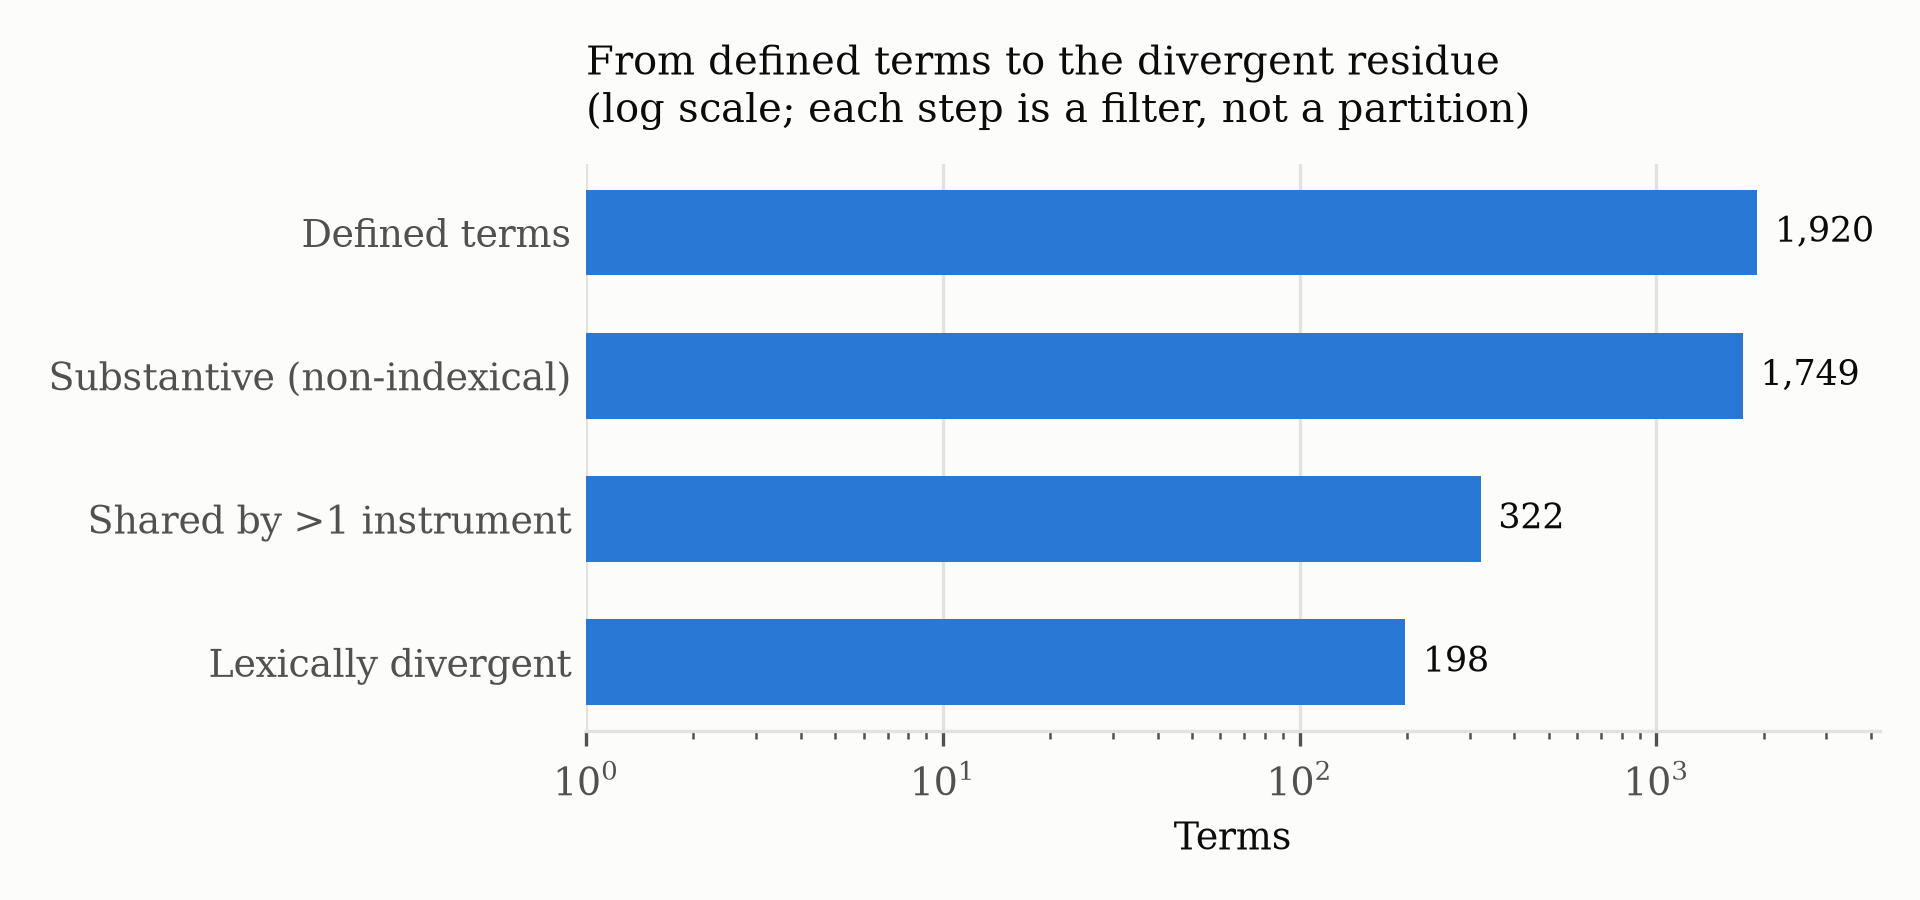
\includegraphics[width=\textwidth]{fig1_funnel.png}
\caption{From all defined terms to the lexically divergent residue. Each
step is a filter: 1{,}920 defined terms, 1{,}749 of them substantive, 322 of
those shared by more than one instrument, 198 of which diverge lexically.}
\label{fig:funnel}
\end{figure}

\begin{table}[t]
\centering
\small
\begin{tabular}{lr}
\toprule
\textbf{Measure} & \textbf{Value} \\
\midrule
Distinct defined terms & 1{,}920 \\
Definition occurrences & 3{,}318 \\
Instruments with a parsed definitions article & 214 \\
\midrule
Indexical terms & 171 \\
Substantive terms & 1{,}749 \\
\midrule
Terms defined by more than one instrument & 362 \\
\quad of which indexical & 40 \\
\quad of which substantive & 322 \\
\midrule
Substantive shared terms, lexically identical & 94 \\
Substantive shared terms, near-identical & 30 \\
Substantive shared terms, lexically divergent & 198 (61.5\%) \\
\bottomrule
\end{tabular}
\caption{Definitional structure of the corpus.}
\label{tab:funnel}
\end{table}

Table~\ref{tab:funnel} and Figure~\ref{fig:funnel} give the shape of the
data. Two features deserve comment before any interpretation.

First, \textbf{most defined terms are not shared at all}. Of 1{,}920 terms,
1{,}558 are defined by exactly one instrument. Saudi legislative drafting
is overwhelmingly local: each statute builds its own vocabulary and only 19\%
of terms are touched by more than one instrument. Fragmentation, whatever
its extent, is confined to a small part of the lexicon.

Second, \textbf{indexical definitions dominate the top of any raw ranking}.
The most frequently defined terms in the corpus are ``the Law'' (125
instruments), ``the Regulation'' (118), ``the Minister'' (85), ``the
Ministry'' (75), ``the Authority'' (67) and ``the Council'' (60). All are
indexical. A study that reported these as the most contested terms in Saudi
law would be reporting a drafting convention.

\subsection{Lexical divergence overstates conflict}

\begin{figure}[t]
\centering
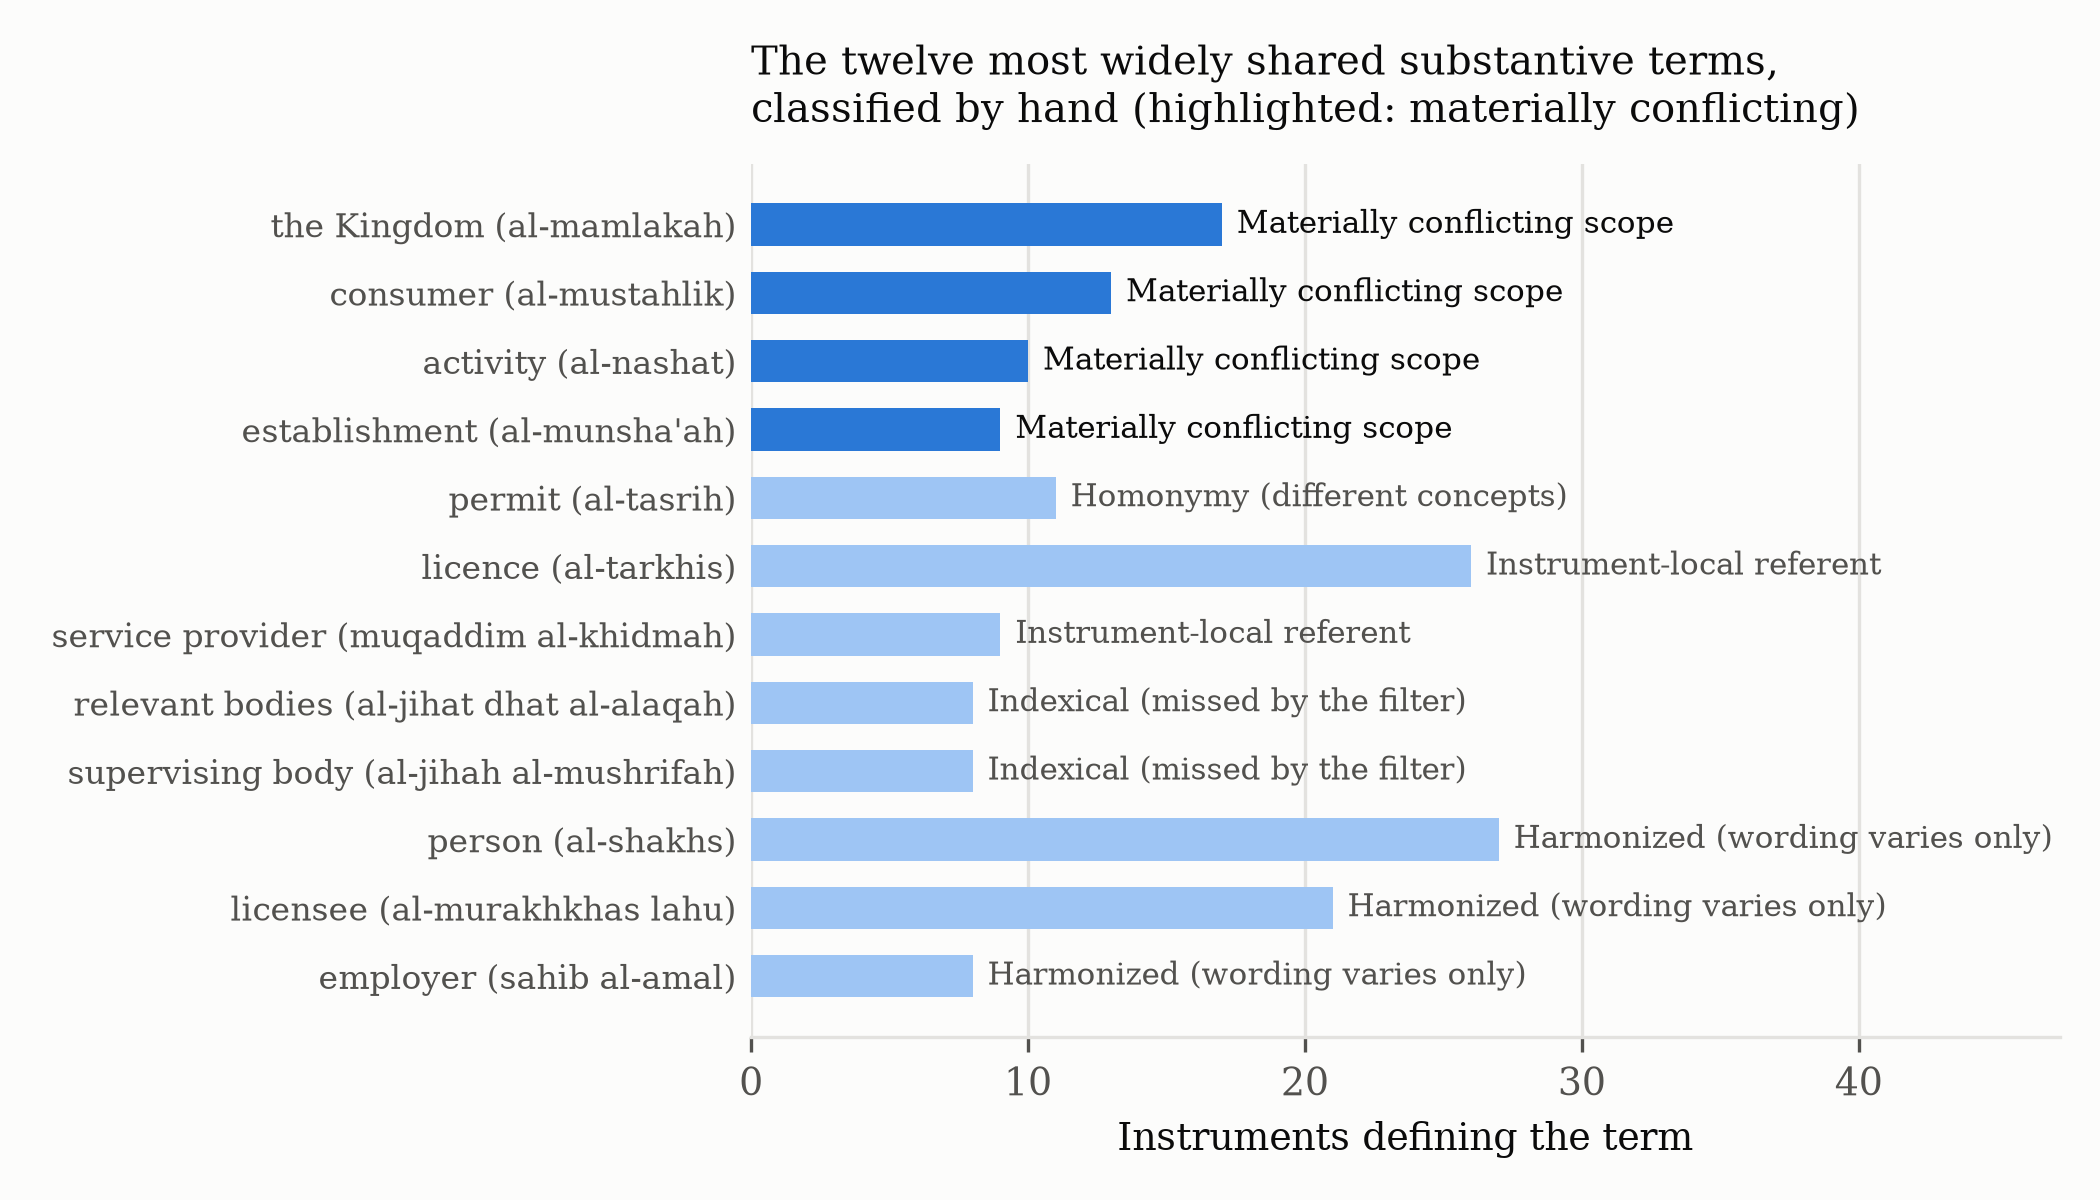
\includegraphics[width=\textwidth]{fig2_adjudication.png}
\caption{The twelve most widely shared substantive terms, classified by hand
across every instrument that defines them. Four carry materially conflicting
scope; the rest diverge in wording, referent or concept rather than in law.}
\label{fig:adjudication}
\end{figure}

Among the 322 substantive shared terms, 198 (61.5\%) are lexically
divergent. Read by hand, that figure does not survive
(Figure~\ref{fig:adjudication}).

Of the twelve most widely shared substantive terms, three are
\textbf{harmonized}: ``person'', ``licensee'' and ``employer'' carry the same
legal content wherever they appear, in wording that varies. ``Person'' is
the extreme case --- 27 instruments, lexical similarity near zero between
some pairs, and no legal difference whatever between ``the natural or legal
person'' and ``any person of natural or legal capacity''.

The adjudication also measures the automatic filter against a hand-read
sample, which is the only recall figure we can offer for it: of the twelve
terms, two turned out to be indexical definitions the filter classified as
substantive, so its recall on widely shared terms is around 83\%. We report
the misses in place rather than correcting them silently, since correcting
them would inflate the filter's apparent accuracy on the very sample used to
assess it.

Two are \textbf{instrument-local}: ``licence'' and ``service provider''
denote the same kind of thing everywhere, an authorisation and its holder,
with each instrument fixing the sector and the issuing body. Two more are
\textbf{indexical} definitions that the automatic filter did not catch ---
``relevant bodies'' and ``supervising body'' each name whichever government
entities the enacting instrument designates.

One is \textbf{homonymy}: ``permit'' covers a temporary agricultural
authorisation in one instrument, an aircraft overflight clearance in
another, and a pre-commencement environmental document in a third. These are
different concepts wearing the same label, which is a feature of natural
language rather than a defect of legislation.

\subsection{The four conflicting terms}

Four terms carry materially different scope for what is recognisably the
same concept.

\emph{Al-munsha'ah} (``establishment''), defined by nine instruments, is the
clearest. The Competition Law and its regulation define it as any natural or
legal person carrying on an economic activity. The Anti-Concealment
Regulation extends it to ``anyone practising an economic activity, including
the sole proprietorship, the company, and any other legal form''. The Labour
Law defines it instead as any undertaking run by a natural or legal person
that employs one or more workers for wages. The difference is not stylistic:
a sole trader with no employees is an establishment for competition purposes
and is not one for labour purposes. Any system --- human or automated ---
that resolves ``establishment'' without asking which statute is speaking
will be wrong for some population of businesses.

\emph{Al-mustahlik} (``consumer''), defined by thirteen instruments, ranges
from a person with credit dealings, in the credit-information regime, to a
residential or commercial consumer in the electricity regime, to a person
transacting electronically in the e-commerce regime. The regimes are
adjacent enough that the divergence has practical consequences for who
enjoys consumer protections in a transaction that spans them.

\emph{Al-mamlakah} (``the Kingdom''), defined by seventeen instruments, is
usually simply ``the Kingdom of Saudi Arabia''. Instruments with an extraterritorial
reach define it as the territory of the Kingdom \emph{including} areas
beyond the territorial waters over which the Kingdom exercises sovereign
rights. For a term that fixes jurisdictional scope, that is a substantial
difference, and it is invisible to anyone reading a single instrument.

\emph{Al-nashat} (``activity''), defined by ten instruments, runs from ``a
type of subsidiary work within a field'' to ``any project or industrial,
commercial or service facility expected to have environmental effects'' to
commercial activity carried on for profit. Here the divergence approaches
homonymy, and we classify it as conflicting because the instruments concerned
regulate overlapping conduct.

\section{Discussion}
\label{sec:discussion}

\paragraph{The measurement problem generalises.}
Any attempt to measure definitional consistency automatically will encounter
both filters described here. Indexical definitions exist wherever
instruments name themselves and their own institutions, which is to say
nearly everywhere; and lexical similarity will always be a poor proxy for
legal identity, in any language. A study that reports an unfiltered figure
is reporting drafting convention plus paraphrase. The size of the gap is
worth stating precisely, because it is easy to overstate: all twelve
adjudicated terms are lexically divergent, and four of them are
substantively conflicting, so within this sample lexical divergence
overstates substantive conflict roughly \emph{threefold}. That ratio is
measured on twelve terms and should not be projected onto the other 310
shared substantive terms, nor onto other jurisdictions; measuring it
elsewhere would be a useful test of whether a similar factor holds.

\paragraph{Harmonisation is tractable.}
The practical implication for legislative drafting is optimistic. If
definitional conflict in Saudi legislation were pervasive, harmonisation
would be a generational project. If it is concentrated in a handful of
high-traffic terms --- establishment, consumer, the Kingdom, activity ---
then a drafting body could address it deliberately, and the corpus makes the
candidate list computable rather than anecdotal.

\paragraph{Consequences for legal AI.}
Systems that answer questions over statutory text must resolve terms, and
the conflicting cases are exactly where naive resolution fails. A
retrieval-augmented system asked whether a sole trader is subject to an
obligation imposed on ``establishments'' will retrieve a definition --- and
which definition it retrieves determines the answer. Term resolution in
legal AI is therefore not a lookup but a choice of governing instrument, and
a system that does not model that choice will be confidently wrong on
precisely the terms that matter most.

\section{Limitations}
\label{sec:limits}

\paragraph{The glossary is parsed, not curated.}
Definitions come from an automatic parser over definitions articles. We
observed occurrences where one definition's text bleeds into the next, and
terms defined outside the definitions article are not captured at all. The
counts here are therefore approximate at the margins.

\paragraph{The indexical filter is a heuristic.}
It is inspectable and we report its misses --- two of the twelve adjudicated
terms are indexical definitions it did not catch --- but it has no measured
precision or recall against a hand-labelled sample. Building that sample is
the obvious next step.

\paragraph{The adjudication is single-annotator and small.}
Twelve terms were classified by one reader. There is no inter-annotator
agreement to report, the classes involve judgement at the boundaries
(``activity'' could be defended as homonymy rather than conflict), and the
finding should be read as a documented reading rather than a measurement.

\paragraph{The sample is chosen by frequency, which may understate conflict.}
The twelve adjudicated terms are those shared by the most instruments, and
frequency selects for generality: widely shared terms tend to be broad
concepts (``person'', ``licence'') that are easy to harmonise or that
diverge only by sector. Genuinely conflicting \emph{technical} terms, shared
by two or three instruments in adjacent regimes, would sit in the tail and
are not examined here. The four-in-twelve figure is therefore a lower bound
on the density of conflict in the shared lexicon, not an estimate of it.

\paragraph{Divergence is not the same as inconsistency.}
Two instruments may define a term differently for good reason, because they
regulate different conduct. Nothing here establishes that the four
conflicting cases are drafting errors; the claim is that they are places
where the same word carries different legal content, which is a fact about
the system that its users need to know.

\paragraph{Coverage.}
Only the 214 instruments whose definitions articles parse cleanly
contribute. Instruments without a definitions article, and those the parser
skipped, are invisible to the study.

\section{Conclusion}

Definitional fragmentation in Saudi legislation is real, narrow, and
measurable. Of 1{,}920 defined terms, most are used by a single instrument;
of the 322 substantive terms that more than one instrument defines, 61.5\%
diverge lexically; and of the twelve most widely shared, four carry
materially different legal scope. The gap between the second figure and the
third is the paper's main methodological claim: measuring statutory
definitional consistency automatically requires separating indexical from
substantive definitions and lexical from substantive divergence, and a study
that does neither will report a number about drafting convention and
paraphrase rather than about law.

The four conflicting terms are, in a sense, the smallest possible finding
and the most useful one. \emph{Establishment} means one thing to the
competition regime and another to the labour regime, and a sole trader falls
on different sides of that line depending on which statute is asking. That is
a fact a practitioner may know and a machine cannot infer --- and it is now,
for this jurisdiction, enumerable.

\ifanon\else
\section*{Declarations}

\paragraph{Funding.} No funding was received for conducting this study.

\paragraph{Competing interests.} The author declares no competing interests.

\paragraph{Ethics approval.} Not applicable. The study involves no human
participants, no animal subjects, and no personal data; it analyses
published national legislation only.

\paragraph{Data availability.} The corpus, its glossary layer, and the
analysis and figure scripts that reproduce every number and figure reported
here are openly available at
\url{https://github.com/Abdullah-m7/saudi-legal-corpus-ai} and archived on
Zenodo under the MIT licence
(\href{https://doi.org/10.5281/zenodo.22019183}{10.5281/zenodo.22019183};
concept DOI
\href{https://doi.org/10.5281/zenodo.22019182}{10.5281/zenodo.22019182}).

\paragraph{Author contributions.} A.~Almohammedi is the sole author and
conducted all aspects of the work.

\paragraph{Legal status.} This paper analyses a non-official research corpus.
Nothing here constitutes legal advice; the binding text of any instrument is
the Arabic original published in \emph{Umm Al-Qura}.
\fi

\bibliographystyle{plainnat}
\bibliography{references}

\end{document}
